\section{Sound and Light! (A Microphone and a Photocell)}
\label{lab_microphone_photocell}

%\makelabheader %(Space for student name, etc., defined in master.tex)

\bigskip

\begin{enumerate}[wide]

\item One place where field effect transistors are useful is in an electret microphone.  An electret is a material that holds a permanent polarization, something like the electric equivalent of a permanent magnet.  This material is mounted on a movable diaphragm that vibrates in response to sound, so that its vibration induces a small oscillating voltage in a nearby electrode.  A convenient way to detect this small voltage is to apply it to the gate of a field effect transistor.  Your microphone already has a transistor built into it.  Connecting the microphone to an external power source and resistor and removing the DC bias with a capacitor as shown produces an AC signal that's easy to measure.  How big is the resulting AC output when you whistle into the microphone?   (Note that the leads of your microphone are polarized; the negative terminal is the one that's visibly shorted to the outside of the capsule.)  
\begin{center}
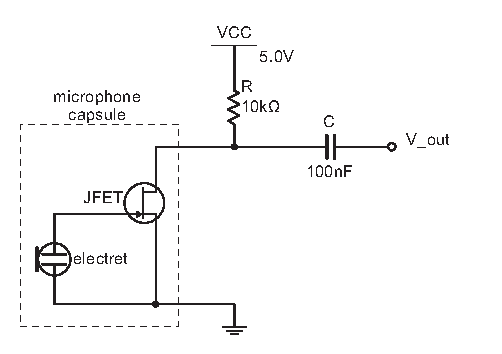
\includegraphics{microphone_photocell/microphone_circuit.eps}
\end{center}

\item The resistor value above was chosen to make the DC output of your microphone about $V_{CC}/2$, which maximizes its AC amplitude.  Suppose the channel of the JFET in your microphone is behaving like a simple variable resistor.\footnote{The JFET is \textit{not} a simple variable resistor, because its $IV$ characteristics are highly nonlinear.}  Based on the AC amplitude you measured above, what is the range of its effective resistance when you whistle into it?

%This next part is better for homework than for the lab, I think.
%\item From the resistance range you just calculated, what would be the amplitude of your microphone's AC output if you used an external resistor $R=470$~k$\Omega$?  How about if you used $R=470$~$\Omega$?  (No need to build and measure these.  In fact, the nonlinear behavior of the JFET means your results would differ significantly from what you calculated, though the AC outputs in both cases would still be pretty small.)

\item The 1~$\mu$F external capacitor you used, in conjunction with the input impedance of your oscilloscope, acts as a filter to eliminate the DC offset from your microphone.  Is it a high-pass filter or a low-pass filter?  Calculate the filter's cutoff frequency.

\item As long as we're playing with detectors, your kits also include a photocell, or ``photoresistor.''  (It's the two-terminal thingy with a squiggly line on 
the top.) This is essentially a resistor made 
\begin{minipage}{0.8\textwidth}
\vspace{.18\baselineskip}
of cadmium sulfide, which is a semiconductor similar to silicon.  The resistivity of this material changes in response to light, 
as incident photons excite charge carriers across the band gap.  What is the resistance of this device in the ambient light of the room?  When you put your thumb over it?  Design and test a circuit that turns a current of 10~mA through an LED on and off  when you pass your hand over a photocell.  (\textit{One-word hint: ``Comparator.''})
\end{minipage}
\begin{minipage}{0.19\textwidth}
\begin{center}
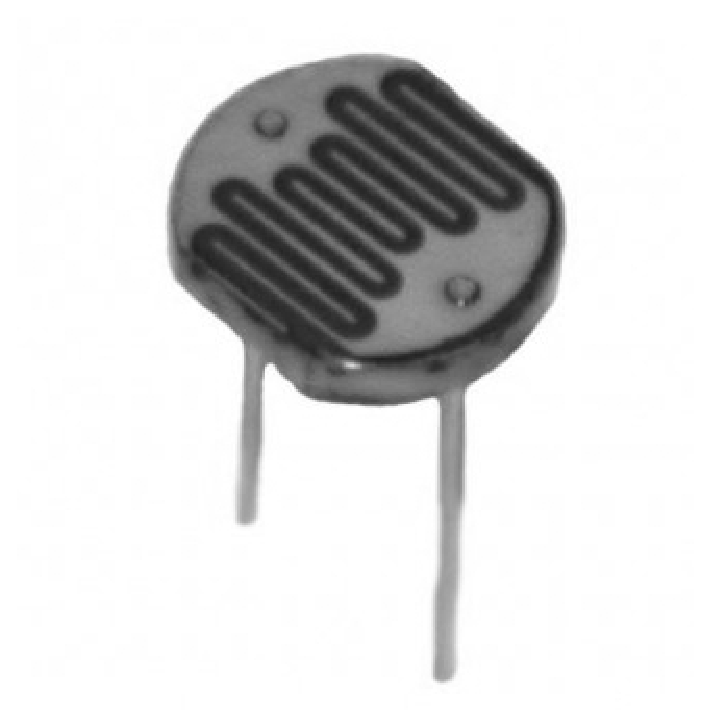
\includegraphics[width=1in]{microphone_photocell/photocell_bw.eps}
\end{center}
\end{minipage}


\end{enumerate}
